\chapter{Mbona Hatcheries Procedures}

\section{Procedures}

%\subsection{Production Schedule, with TimeLine.}

In this section we track the progress of trout from eyed-eggs to fry to fingerlings, see figure ~\ref{fig:EggsFryFingerlings}.

\begin{figure}[H]
  \centering
   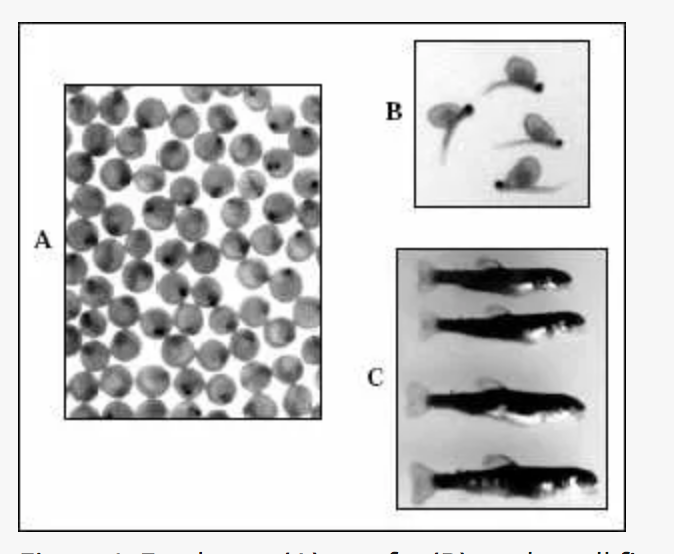
\includegraphics[scale = 0.6]{images/EggsFryFingerlings.png}
  \caption{What to look for: A) Eyed-Eggs, B) Sac-Fry, C) Fingerlings}
   \label{fig:EggsFryFingerlings}
\end{figure}

After this they spend the rest of their time in in the hatchery ponds as pre-sale growing fish.
In what follows we track the trout from Haching to sale giving feeding and cleaning schedules 
that must be followed.

\subsection{Preparation of Hatchery for new batch of eggs}

Make sure the fish food store is replenished. Purchase replacements from AVI feeds in Pinetown, 
see contact details ~\ref{tab:SupplierContactDetails}, who will deliver to Hopewell in Howick.
The current food range is outlined in the feed table ~\ref{tab:TablesFishFood}. This table is
just a suggestion, The suppliers of the feed should be consulted for their recommendation.

\begin{table}[H]
  \centering
   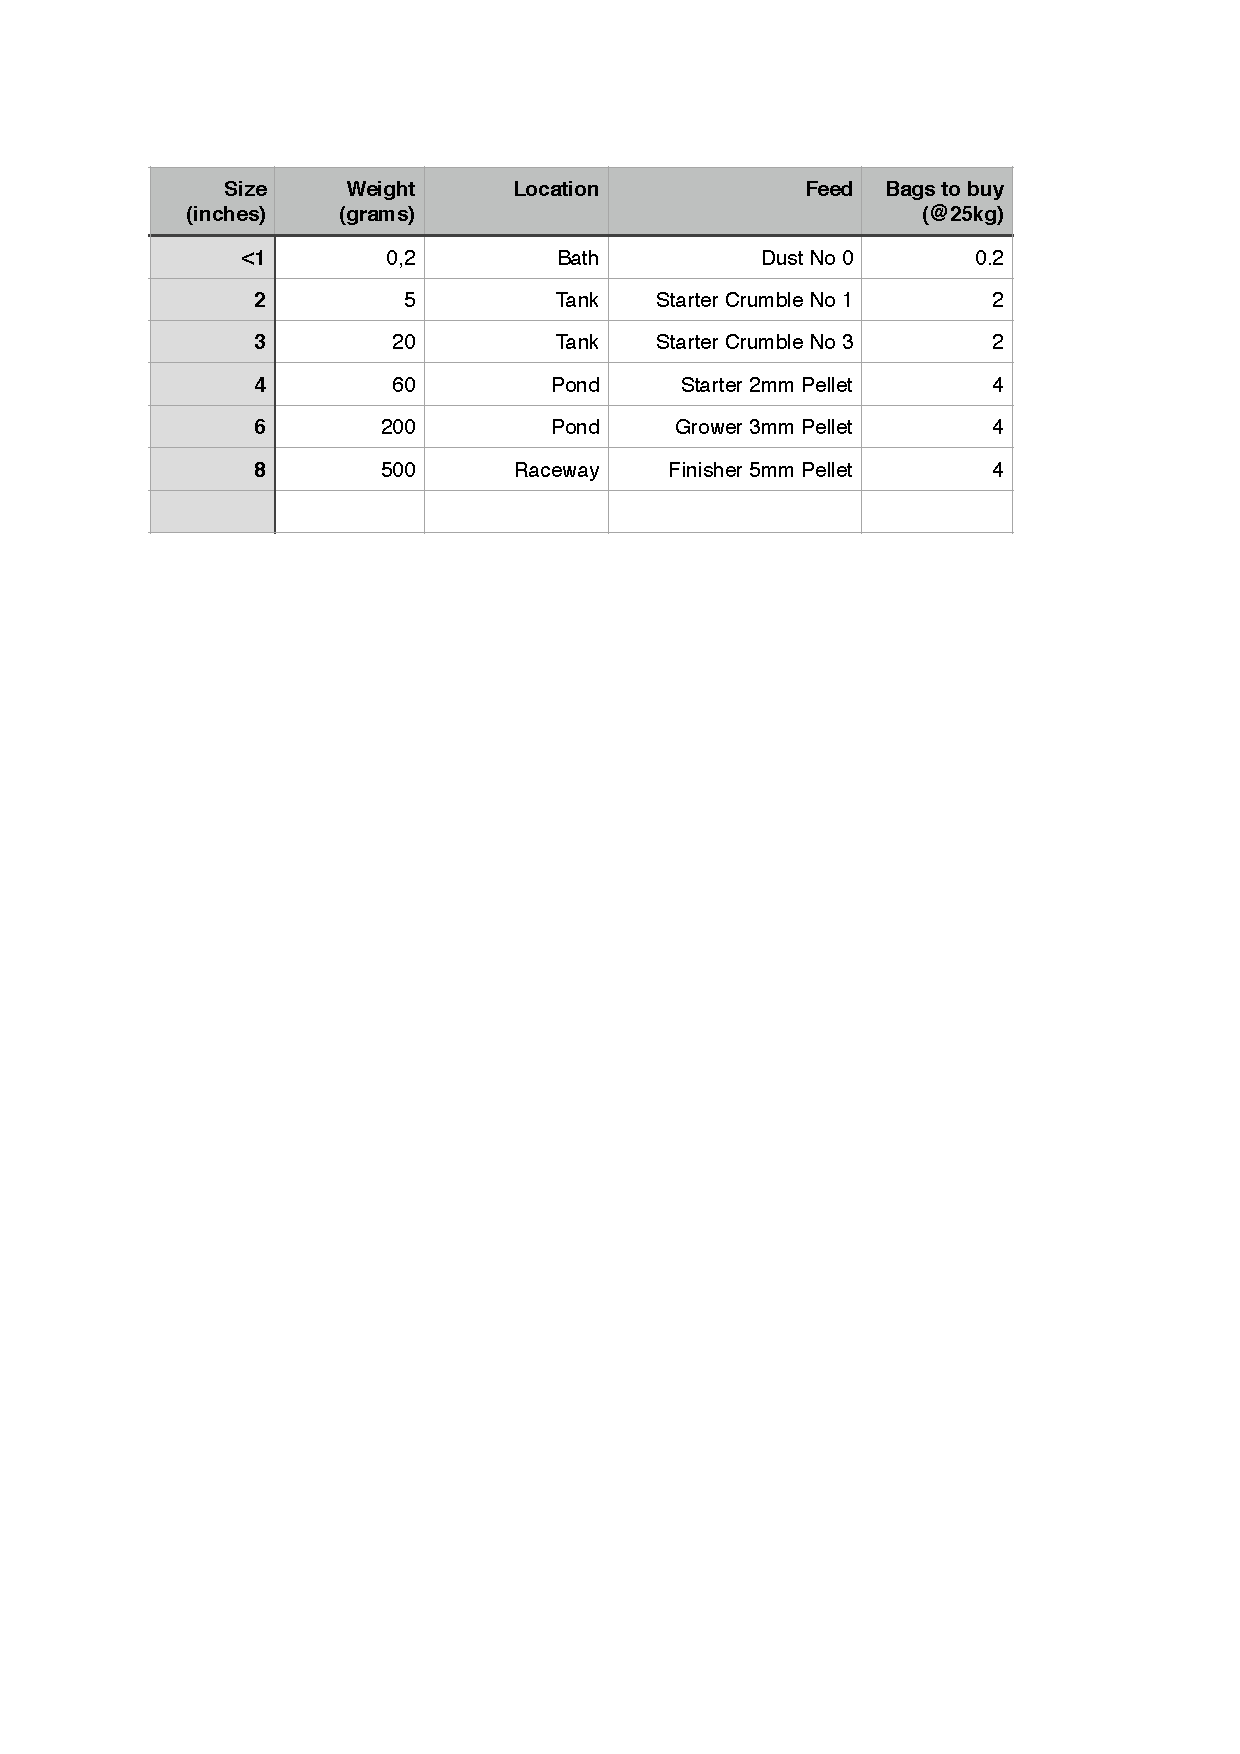
\includegraphics[scale = 0.9]{tables/TablesFishFood.pdf}
   \caption{Fish Feed: showing feed type to match different stages} 
   \label{tab:TablesFishFood}
\end{table}


Two weeks before the eggs arrive start with the following repairs and maintenance:  \marginpar{-2 \W}
\begin{itemize}
   \item Scrub three baths with abrasive pads \& Handy Andy
   \item Clean \& service in-feed pipes
   \item Clean \& service out-flow filters
   \item Check drain plugs \& safety locks
   \item Check \& repair mini vacuum cleaner
   \item Check the following equipment:
   \begin{itemize}
      \item 220 volt light globes in hatching room
      \item Roller blinds \& window covering
      \item Egg tweezers \& dead egg removal pipe \& bird feathers
      \item Head lamps \& batteries
      \item Digital scale
      \item Thermometers
      \item {\bf V} channel egg counter
      \item PVC gloves
      \item Egg transporting box
   \end{itemize}
\end{itemize}
   
Two or three days before arrival of eggs: \marginpar{-0.5 \W}
\begin{itemize}
   \item Scrub down all baths \& equipment again with Hibitane
   \item Position square egg trays in baths \& start water flow
\end{itemize}

On the day of collection \marginpar{0 \W}
\begin{itemize}
      \item Take egg transporting box, thermometer \& note pad.
      \item Buy ice in Howick, load transporting box \& pack spare ice in cool bag
\end{itemize}


\subsection{Transportation of eggs}

At the end of May about 10000 {\bf Eyed Eggs} are purchased from a Hatchery in 
Underberg, see the contact details table ~\ref{tab:SupplierContactDetails} .

Eggs are transported in a polystyrene box with trays of ice above and below the tray of eggs.
    The temperature in the box should be about  \SI{4}{\celsius}.

Eggs at  \SI{4}{\celsius} can be boxed for as long as 96 hrs (4 days).
The hatch-out-rate guarantee should be about 90\%.
The expected time to hatch out at  \SI{10}{\celsius} should be between 6 and 7 days.
    
Once the eggs have arrived at {\bf 0 \W} (weeks after arrival) they progress from 
hatching baths to fingerling tanks to fish ponds the schedule of which is outlined below:


\subsection{Egg handling on arrival}

On arrival at Mbona Hatcheries the eggs have to be tempered and  counted.
 \marginpar{0 \W \\ $1^{st}$June}

    
The tempering process requires increases the temperature of the eggs 
               to the temperature of the water in the incubation trays in a slow and regular manner. 
               The recomendation is  \SI{1}{\celsius} per hour.
               The temporing is accomplished as follows:
         \begin{itemize}
             \item[] Measure boxed eggs temperature.
             \item[] Half fill a bucket.
             \item[] Add ice or iced water to bring down bucket water temperature to egg temperature.
             \item[] When the two temperatures are equalised remove the ice from the bucket.
             \item[] Carefully add eggs to bucket and rehydrate eggs.
             \item[] Slowly bring the bucket temperature up to incubation tray temperature 
                        by adding small amounts of Mbona water from the baths to the bucket.
             \item[] aim for an increase of  \SI{1}{\celsius} per hour.
         \end{itemize}
         
Once the eggs have rehydrated the counting of the eggs can be accomplished by weighing a batch of 200 eggs, $W_B$, that are counted from a pharmacy tablet-counting device and then weighing the remaining eggs, $W_R$, in the rehydration bucket and computing the number of eggs received according to:
            
    $$ N_{eggs} = 200(1 + \frac{W_R} {W_B} ) $$
    
     In the past counting was done by the supplier in the presence of the customer so there was no need to recount on arrival at Mbona. 
     
     

\subsection{Hatching Bath Procedures}

  

\subsection{Hatching of Eyed Eggs}

Once the eggs have been transferred to the hatching trays they will take two weeks to hatch.
During this time white eggs (eggs that have died) must be removed from the hatching tray by
means of a suction straw. If this is not done regularly then the dead eggs will contaminate the live ones.  
\marginpar{2 \W}

After about two weeks, depending on water temperature, the eggs will hatch to produce sac-fry 
which will float away from the egg clutch and 
possibly spill out of the hatching tray into the hatching bath. These sac-fry will feed from their sac for another two weeks. 

After this the fry must be taught to feed. This is done by sprinkling food dust, see table ~\ref{tab:TablesFishFood}, on the water surface with a "plastic" water flow inhibitor in place
so that the food dust does not get expelled from the bath before the fry have fed.
\marginpar{4 \W}

In the beginning this feeding must occur at least {\bf SIX} times a day whilst the fry are still in the baths.
After 2 weeks of feeding the feeding rate can be reduced to {\bf FOUR} times a day for another 2 weeks.
Note that when the fry are young they must be fed small amounts and often so as to maintain equal growth rates amongst the fry and thus reduce canabalism. 

After feeding, some food dust will sink to the bottom of the bath and this sediment must be cleaned 
regularly by  vacuuming the bottom of the bath with the mini vacuum machine.
     
 \subsection{Relocation of fry from Baths to Tanks}
 
 As soon as the fry learn to feed by themselves the Tanks must be prepared to receive the fry.
 All four tanks must be cleaned with diluted Chlorhexiden Gluconate, (Hibitane). Read the 
 instructions to get the dilution proportions. 
 The sides of the tanks must be brushed and broomed and flushed repeatedly. 
 The water must be running a few days before the fish arrive. 
 \marginpar{6 \W}
 
 When the mortality rises in the Baths move the fry to tanks, 
 Use tanks 2 and 4 with {\bf runts} in tank 3.
 Use tank 1 for overflow from 2 and 4.
 Use buckets and the displacement method to count and record the number of fry moved.  
\marginpar{8 \W}

The fry will remain in the tanks for two months. During this time they must be fed with
 starter crumble, see the feed table ~\ref{tab:TablesFishFood}.

\begin{itemize}
          \item twice daily for 4 weeks using starter crumble no 1
          \item twice daily for 4 weeks using starter crumble no 3
\end{itemize} 

 The amount of food to feed can be estimated from the following entry in the 
 Trout in the Classroom website \cite{tic}.
 Assuming 1000 baby fish feed them approximately the following amount of food each day:

\begin{itemize}
\item fish starting to swim up: feed very little (use dust number 0).
\item fish just out of hatch box: 1.5 grams. (use dust number 0)
\item fish approx. 1 inch: 6 grams. (use starter crumble 1)
\item fish approx. 1.5 inch: 17 grams of food (use starter crumble 3).
\item fish approx. 2.25 inch: 55 grams of food (fish ready for transfer to ponds).
\end{itemize}


\subsection{Relocation of fingerlings from Tanks to Ponds}

1 week before the fry reach fingerling stage the ponds must be prepared to receive them.
Use the same technique to clean the ponds. Make sure the ponds are clean and water has
been running for at least two days before transferring the fingerlings.
\marginpar{15 \W}

    Use the gutters and count and transfer the fingerlings to the ponds.
    measure the average length using a 10\% sample of the fingerlings transfered.
    Transfer into pond 1 and 2 with overflow to pond 3   
    \marginpar{16 \W}
    
    
    feeding schedule, see the feed table ~\ref{tab:TablesFishFood}.
        \begin{itemize}
          \item twice daily for 4 weeks using 2mm pellets
          \item twice daily for 4 weeks using 3mm pellets
          \end{itemize}
     after this the fish are ready to move to dams 
     \marginpar{24 \W}

\subsection{Feeding Schedule for growing fish}

When the fish are in the ponds they should be fed according to their total weight per day.
Assuming optimal temperatures between \SI{12}{\celsius} and \SI{18}{\celsius}, they should be fed
$2.5\%$ of their body mass. This amount should be split in two and the growing fish should be fed twice daily.

Below \SI{10}{\celsius} the daily food allowance should be droped to $1.5\%$ of total body mass and below
\SI{5}{\celsius} it should be reduced further to $1\%$ of body mass.

Above \SI{20}{\celsius} the daily food allowance should also be reduced since at this temperature the fish become too lethargic to feed.

The weight, $W$, of a fish can be estimated from its length and girth as follows

\begin{itemize}

\item[] {\bf Imperial} $W$ in pounds, $L$ and $G$ in inches:
$ W  = \frac{1}{800} \times L  \times G^2 $

\item[] {\bf Metric} $W$ in grams, $L$ and $G$ in centimetres.
$ W  =   \frac{450}{800} \times L  \times G^2 $

\end{itemize}

In table ~\ref{tab:TablesWeightComputation} you will find example computations for various fish dimensions

\begin{table}[H]
  \centering
   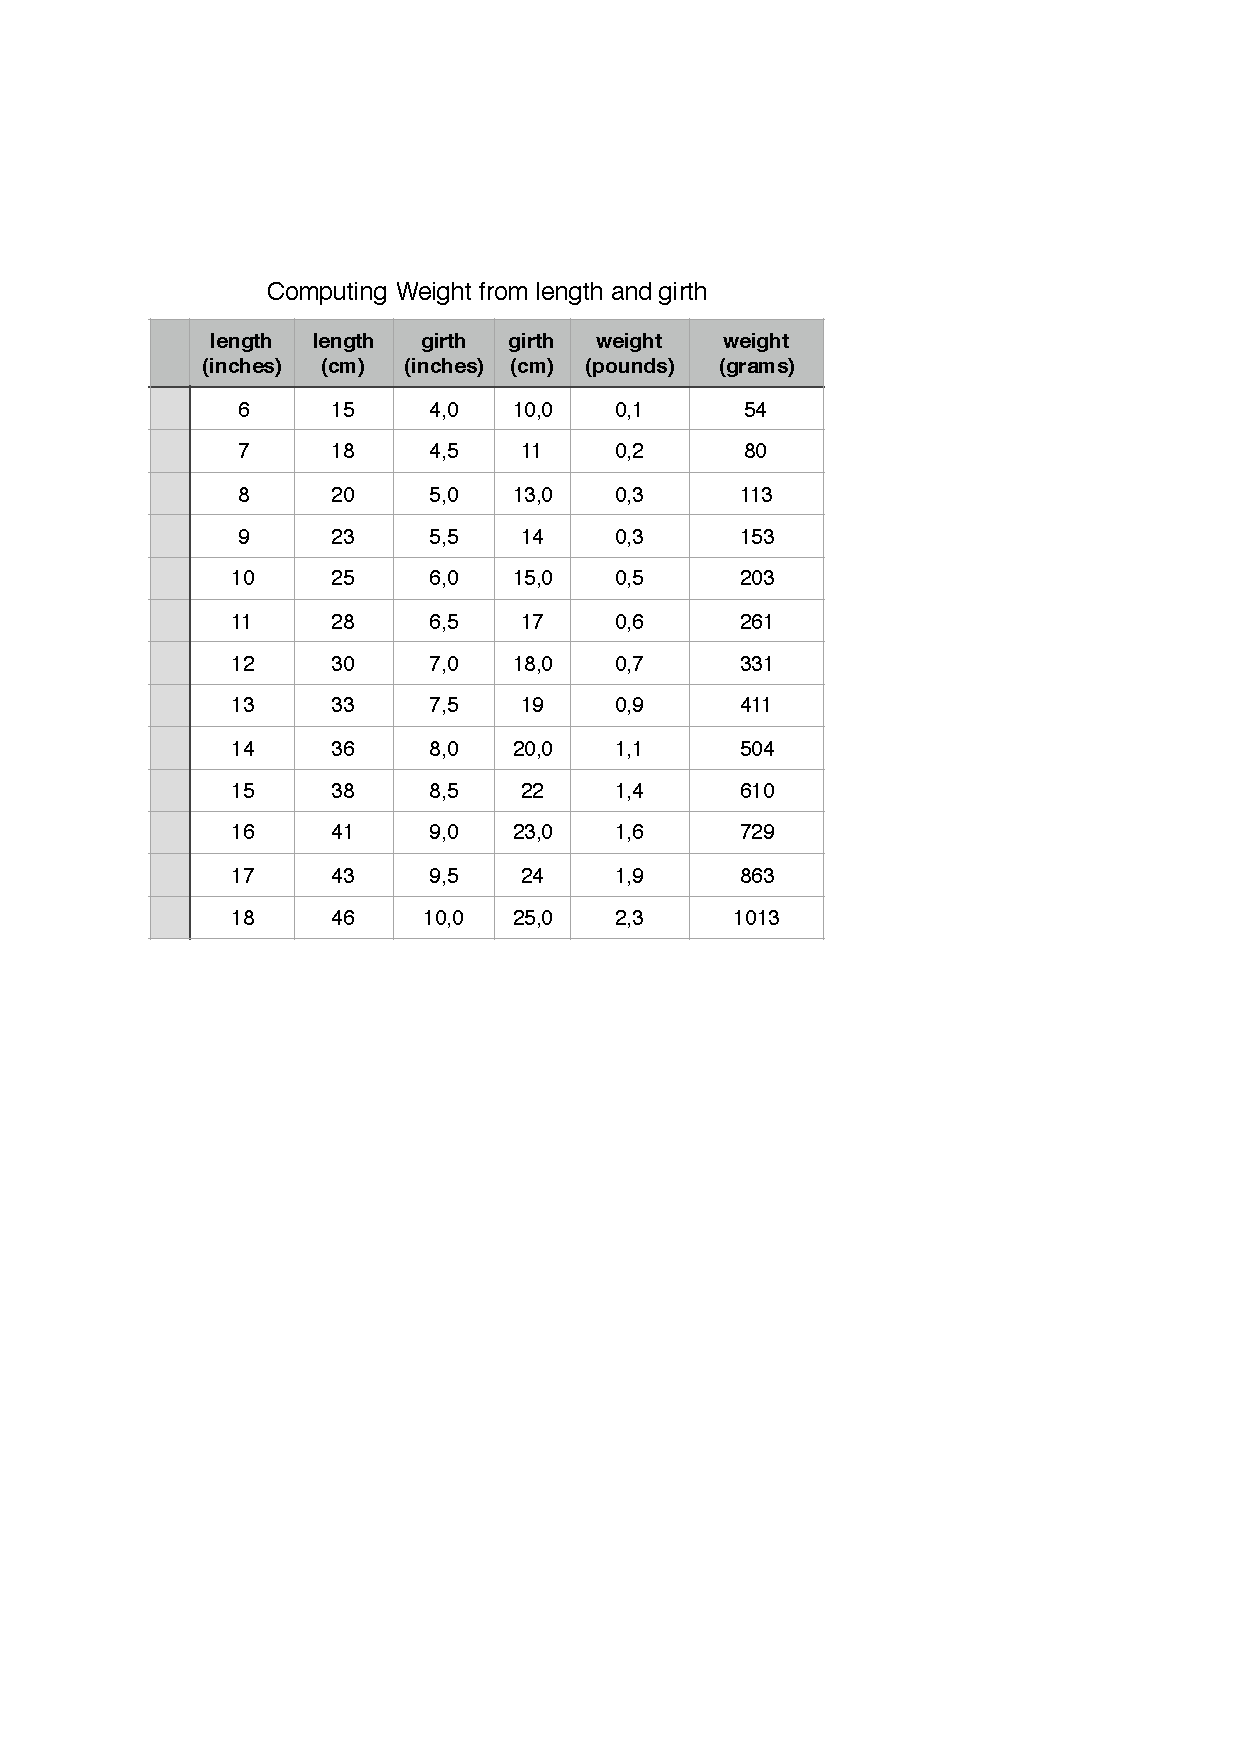
\includegraphics[scale = 0.8]{tables/TablesWeightComputation.pdf}
   \caption{Computing weight from length and girth, $W \approx L \times G^2$}
   \label{tab:TablesWeightComputation}
\end{table}




\subsection{Moving Stock Fish to Dams}
   
    When the fish in the ponds reach an average length of 6 to 7 inches they are ready to
    be sold to customers or used to restock Mbona dams. Customers must be contacted
    timeously so that orders can be taken and expected delivery dates agreed upon and 
    the fishing committee must meet to decide on which dams are to be restocked.
    
    Prices for live fish are set annually. Since the Mbona operation is {\bf non-profit}, prices
    are kept just below market value and sales are limited so that Mbona can stock their
    own dams adequately. Current prices are shown in table ~\ref{tab:TablesFishPrices}.
    
    \begin{table}[H]
  \centering
   
\includegraphics[scale = 0.8]{tables/TablesFishPrices.pdf}
   \caption{Selling Price for Mbona Fish, the six inch price is set annually and
   the price of the larger fish increases 10\% per inch and the price per fish is
   rounded to the nearest rand.}
   \label{tab:TablesFishPrices}
\end{table}
    
    Stock fish are counted and transported using a 600 litre tank mounted on 
    an Mbona Isuzu with oxygenator attached.  The number of fish the tank can  
    accommodate depends on the average size of the fish as outlined in the table ~\ref{tab:TransportationNumbers}.
    
    \begin{table}[h]
  \centering
  \begin{tabular}{|c|c|}
    \hline
    length & number   \\ \hline
    7 inch & 700  \\ \hline
     8 inch & 400  \\ \hline
      9 inch & 300  \\ \hline
       10 inch & 250  \\ \hline
  \end{tabular} 
  \caption{Numbers versus Length for 600 litre vessel.}
  \label{tab:TransportationNumbers}
\end{table}

Live fish that are not sold are used to stock the Mbona dams. The number of live fish a dam can support
depends on the surface area of the dam and the size of the fish. In table ~\ref{tab:TablesDamCapacity} we
show dam capacities for a range of fish sizes. In the last column we show suggested proportional stocking
figures assuming 1000 fish were available for dam stocking. Naturally these numbers are not cast in stone
as dams may not be in a fit condition to receive stock fish. For example,Holbeck may be silted up and
Emerald may be empty.

\begin{table}[H]
  \centering
   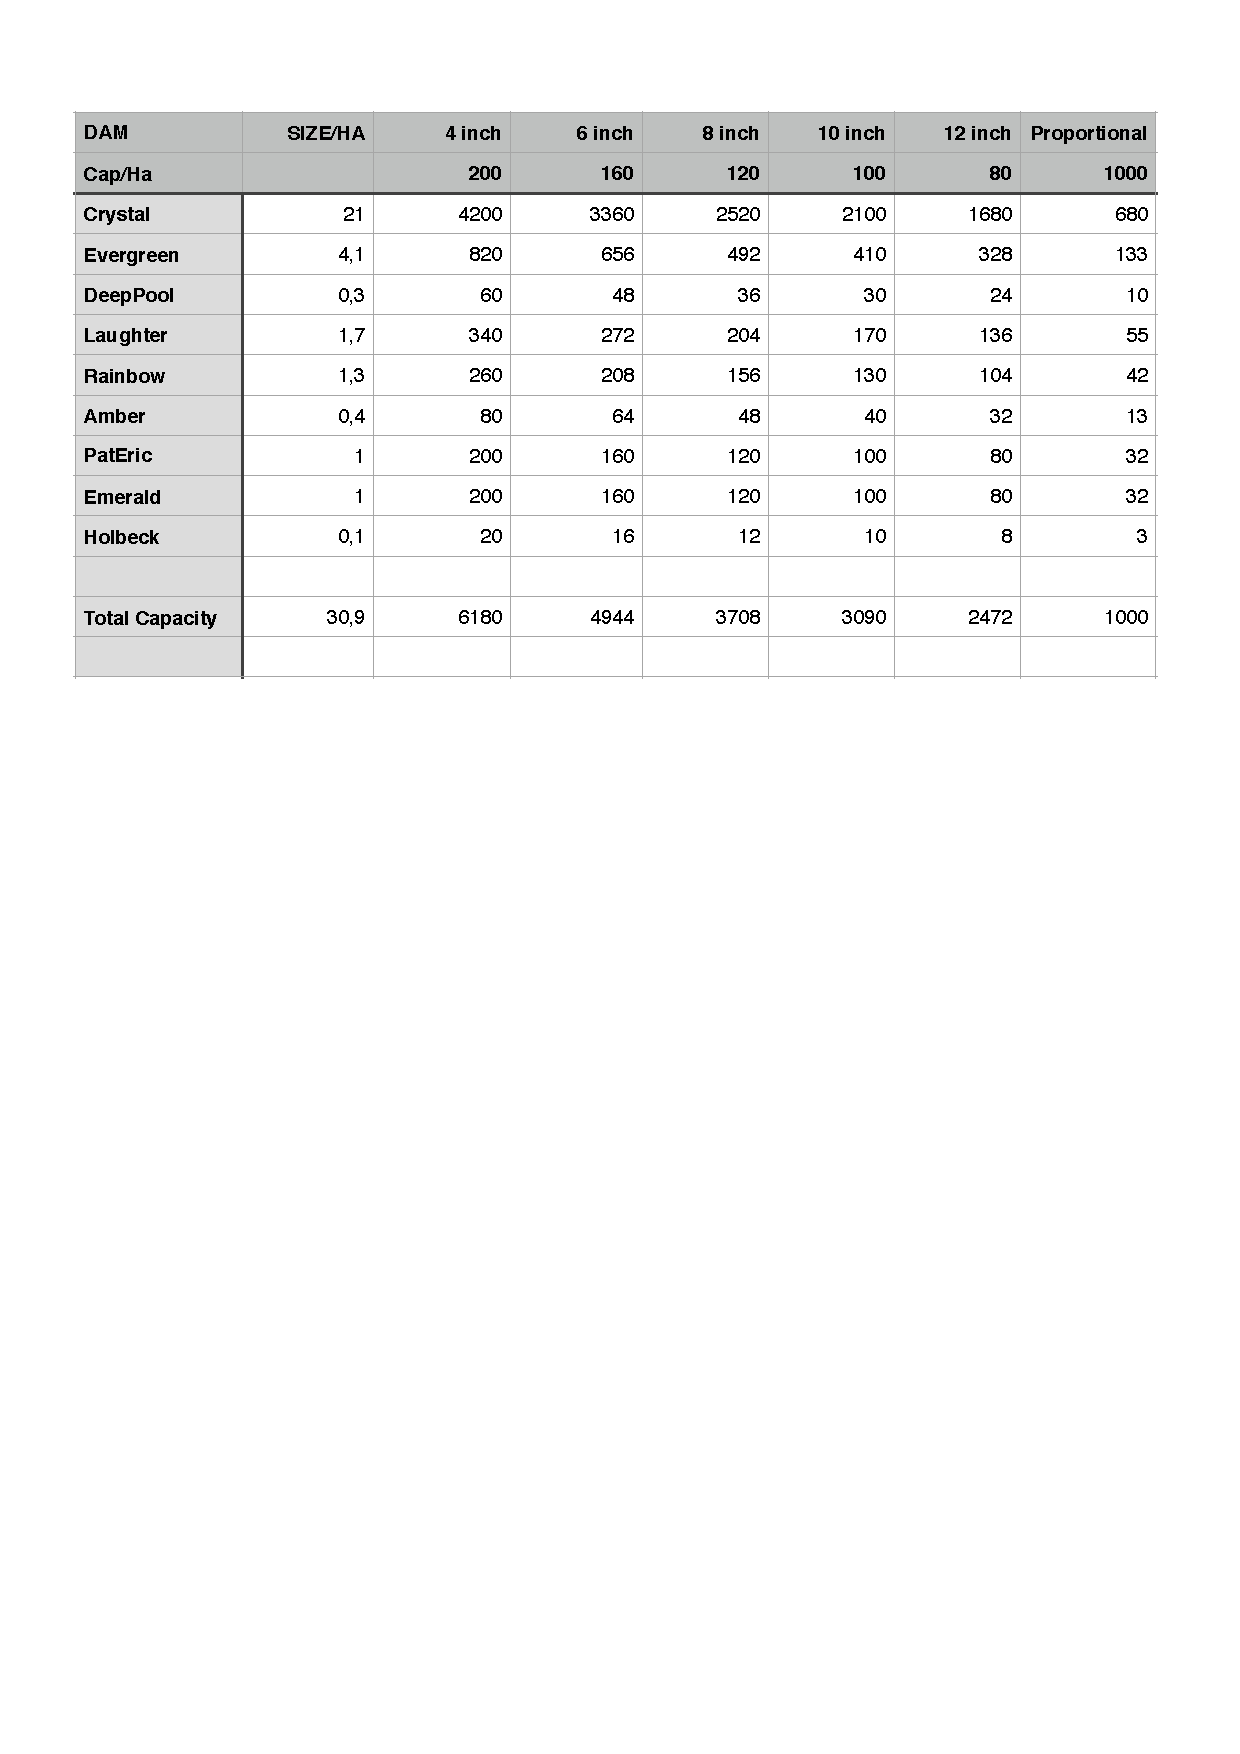
\includegraphics[scale = 0.7]{tables/TablesDamCapacity.pdf}
   \caption{Dam Capacities on Mbona, Each column shows the dam capacities dependent on
   the current size of the stock fish. The last column shows suggested proportional allocation
   assuming 1000 stock fish are available}
   \label{tab:TablesDamCapacity}
\end{table}



\subsection{Hatchery Staff Duties}

\subsubsection{In preparation for egg arrival}

\begin{itemize}
\item When informed of a pending fish delivery, lay out \& check \& clean all delivery equipment.
\item Pack all fish transporting equipment way after use 
\item Report any damaged or lost equipment to management.
\end{itemize}


\subsubsection{During Incubation and sac-fry growth}

\begin{itemize}
\item remove white eggs {\bf three} times per day.
\item make sure baths are clean, just sweep in preparation for hatching.
\item when teaching fry to eat, use very small amounts of dust and fry must be seen breaking the water surface when feeding.
\item Baths must be vacumed a half hour after each feed.
\end{itemize}

\subsubsection{During Growth Period}

\begin{itemize}
\item Feed fish daily according to Size - Quantity - frequency chart.
\item Vacuum clean tanks and ponds after each feed.
\item Keep pond nets in good repair
\item Inspect all fencing \& keep grass cut under \& around electric fence.
\item Keep large \& small catch nets in good repair.
\item Cut grass and keep hatchery area \& hatchery room neat \& tidy at all times.
\item All long catch net \& vacuum poles to be cleaned \& stored on racks
\end{itemize}

\subsubsection{At all times}

\begin{itemize}
\item Keep all fish transporting equipment clean \& stored under cover 
\item Report any broken or damaged equipment to management same day.
\item Report any predator activity, otter or birds of prey, to management same day.
\end{itemize}





\newpage
\section{Mbona Hatcheries Maintenance and Repair}

Maintainance and repair projects as of March 2019 (completed projects marked \checkmark).

\subsection{Hatching room}     

\begin{itemize}
\item Repair bath 2 in-feed pipe
\item Make good all three bath outlets and make adjustable drains. 
\item Make 3 PVC/F-glass mesh filter curtains  
\item Stop leaks in drain out-pipes
\item Sort 220v lighting in hatching room
\end{itemize}

\subsection{Main pond area}     
\begin{itemize}
\item Complete clay repair and gravel of raceway pond.    
\item Complete fencing and gates to new extension   \checkmark
\item Reroute electric fencing \checkmark
\item Run water feed pipe to new area off main 3 pond feed \checkmark
\item Replace small fingerling tank with larger model.
\end{itemize}

\subsection{Shade cloth cover}  
\begin{itemize}
\item Replace and reset gum poles  \checkmark
\item Replace shadecloth \checkmark 
\item Replace swimming pool hose sections where necessary \checkmark
\item Build, using old fencing standards, adjustable drain pipe stands
\item Do 12 volt night light bug catch test with white plastic \checkmark (not successful)
\end{itemize}


\subsection{Syphon water feed from Crystal}
\begin{itemize}
\item  Pull up 2 x 70mm syphon pipes and replace filters \checkmark
\item Move 3 syphon inlets and main water inlet 18 meters further from wall
\item Build mud anchor and substantial top float with nylon rope-pulley lifting system for maintenance.
\item Box and cover 3 x vacuum break valves at Crystal edge for quick access
\end{itemize}


\subsection{Oxygenator}
\begin{itemize}
\item Reseat IBR roof \checkmark
\item Remove T from North 70mm pipe and extend  \checkmark
\item Sort distributor tray or trays \checkmark
\item Check bottom of bath outlet drain \checkmark
\item Re-concrete beneath oxygenator to prevent undermining \checkmark
\item Box and lid 2 x 70mm syphon pipe taps and hose connect points for quick access 
\item Extend and secure steel inspection ladder
\item Gravel South side walk area against wall 
\item Paint oxygenator
\end{itemize}


\section{Budget proposal}

This section requires further development by the fishing committee.

\begin{table}[H]
  \centering
  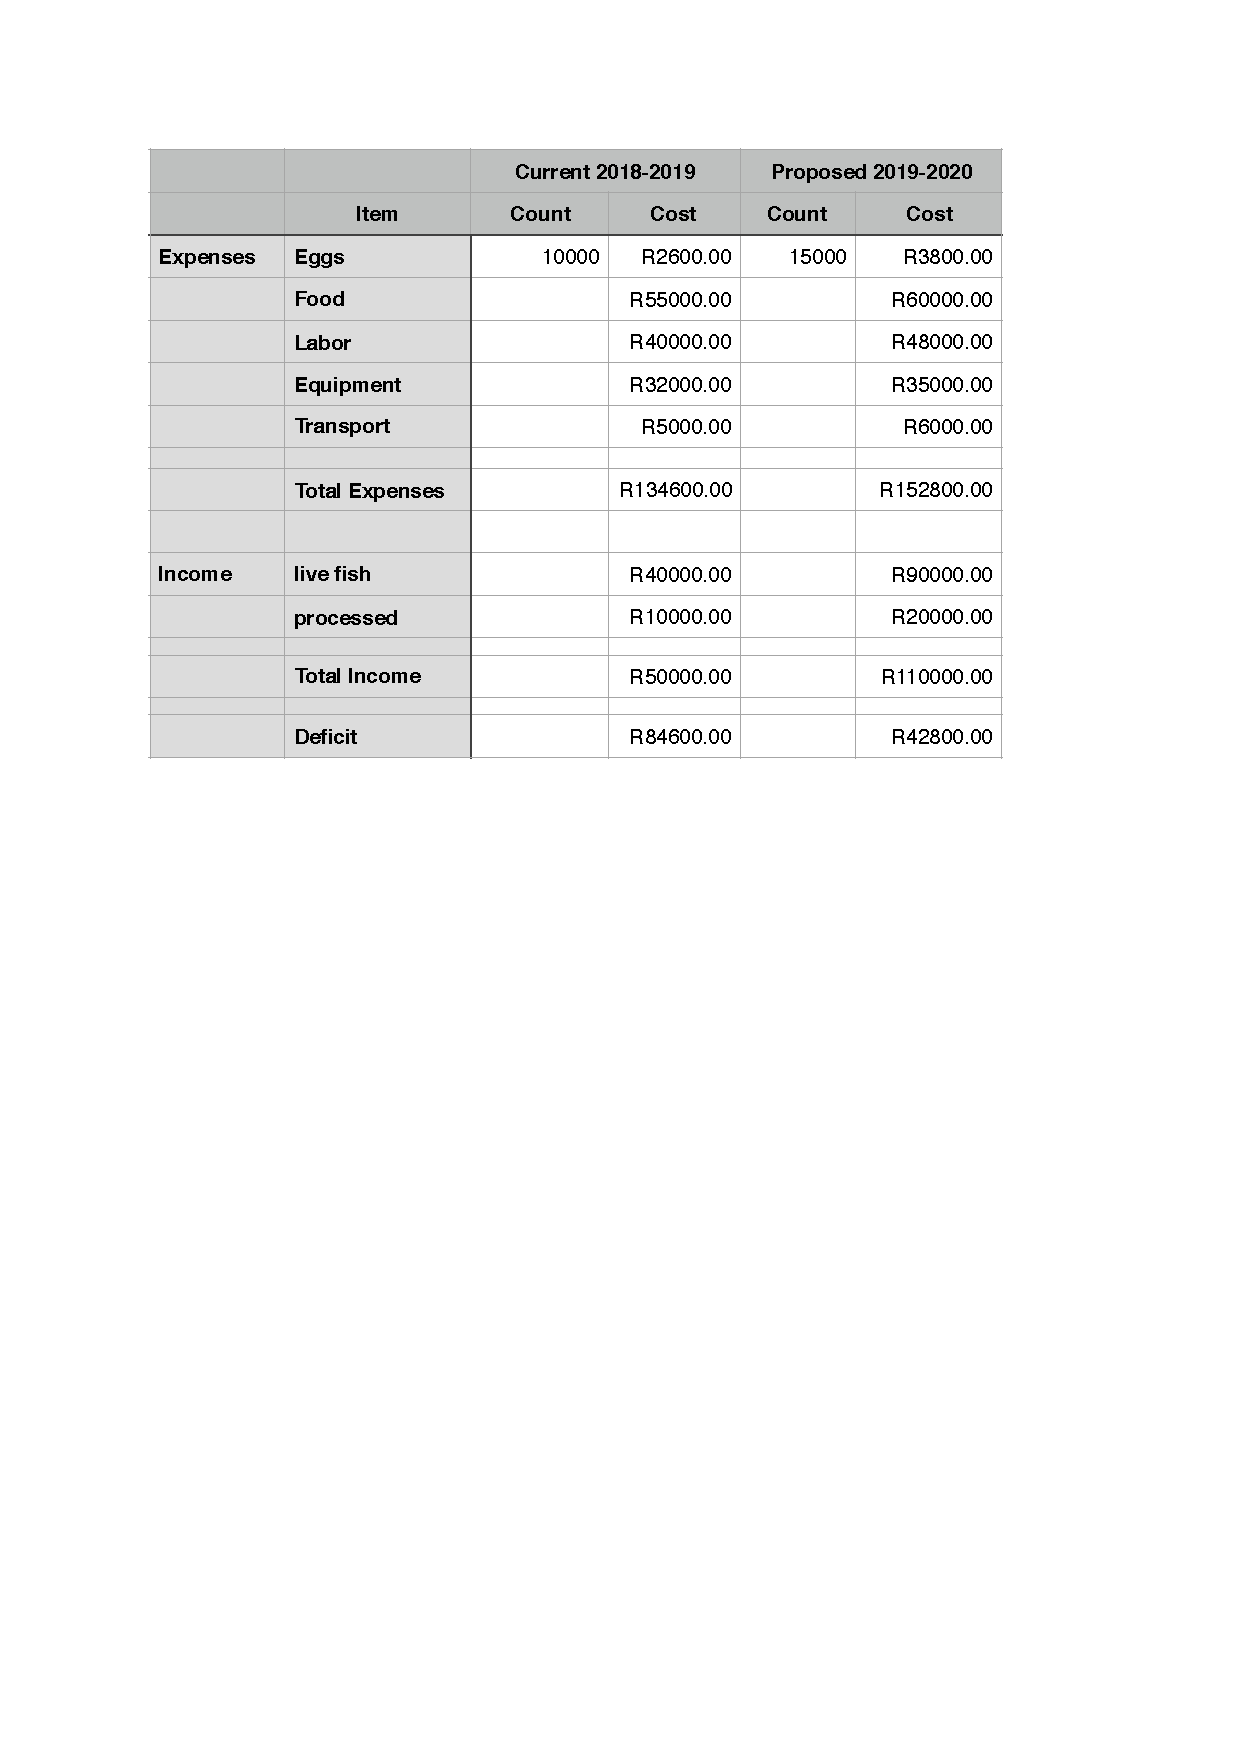
\includegraphics[scale = 0.9]{tables/TablesBudget.pdf}
   \caption{Possible Budget proposal for next season.}
  \label{tab:Budget}
\end{table}
 


